\documentclass[usenatbib]{mnras}
\usepackage[T1]{fontenc}
\usepackage{ae,aecompl}

\usepackage{graphicx}	% Including figure files
\usepackage{amsmath}	% Advanced maths commands
\usepackage{amssymb}	% Extra maths symbols
\usepackage{subfig}
\usepackage{array}

\usepackage{multirow}
\usepackage{multicol}
\usepackage{blindtext}
\newcolumntype{?}{!{\vrule width 1pt}}
\newcommand{\Msun}{\,{\rm Mpc}$_{\odot}$\,}
\newcommand{\Mpch}{\,{\rm Mpc}\,\ifmmode h^{-1}\else $h^{-1}$\fi}
\newcommand{\kpch}{\,{\rm kpc}\,\ifmmode h^{-1}\else $h^{-1}$\fi}
\newcommand{\kpc}{\,{\rm kpc}\,}


\title[Dark matter halo shapes at $z=0$] {Dark matter halo shapes at
  $z=0$ in the Auriga simulations} 
\author[Jesus Prada,  Jaime E. Forero-Romero, Volker Springel ]{
Jesus Prada,$^{1}$\thanks{E-mail: jd.prada1760@uniandes.edu.co}
Jaime E. Forero-Romero,$^{1}$
Volker Springel$^{2}$
\\
% List of institutions
$^{1}$Departamento de F\'isica, Universidad de los Andes, Cra. 1 No.
18A-10, Edificio Ip, Bogot\'a, Colombia\\
$^{2}$Max-Planck-Institut f\"ur Astrophysik, Karl-Schwarzschild-Str. 1, D-85741 Garching, Germany\\
}

% These dates will be filled out by the publisher
\date{Accepted XXX. Received YYY; in original form ZZZ}

% Enter the current year, for the copyright statements etc.
\pubyear{2019}

% Don't change these lines
\begin{document}
\label{firstpage}
\pagerange{\pageref{firstpage}--\pageref{lastpage}}
\maketitle

% Abstract of the paper
\begin{abstract}
We present shape measurements of Milky Way sized dark matter halos at
redshift $z=0$ in a suite of 30 zoom simulations from the Auriga
project. 
We compare the results in full magnetohydrodynamics against dark
matter only simulations. 
We find a strong influence of baryons in making dark matter halos
rounder at all radii compared to its dark matter only counterparts.
At distances $\lesssim 30$ kpc, rounder dark matter distributions
correlate with extended massive stellar discs and low core gas 
densities.  
We measure the alignment between the halo and the stellar disc at
different radii and find almost perfect alignment at
$0.25R_{200}\sim56$ kpc.    
In some cases the alignment significantly changes as a function of
radius implying that the halo shape twists; 
this effect correlates with extended stellar discs and
low gas densities and is almost absent in the dark matter only
simulations.  
In a comparison against observational constraints we find that $20\%$
of halos in our sample are consistent with observational results derived
from the Pal 5 stream that favor an almost spherical shape.
Including baryons is a required element to achieve this
level of agreement. In contrast, none of the simulations (dark matter
only nor with baryons) match the constrains derived from the
Sagittarius stream favoring an oblate dark matter halo.
\end{abstract}

% Select between one and six entries from the list of approved keywords.
% Don't make up new ones.
\begin{keywords}
galaxies: evolution --- galaxies: formation --- galaxies: haloes ---
dark matter
\end{keywords}

%%%%%%%%%%%%%%%%%%%%%%%%%%%%%%%%%%%%%%%%%%%%%%%%%%

%%%%%%%%%%%%%%%%% BODY OF PAPER %%%%%%%%%%%%%%%%%%

\section{Introduction}

Our physical picture of the Universe as a whole has be shaped by
accurate observations and modeling of our own Galaxy. 
Explaining the matter budget and kinematical state of the Milky Way
(MW) is  equivalent to figuring out its formation process in a
cosmological context. 
As a first approximation, the MW morphology and
separation into global kinematically coherent components, such as its
disc and bulge, can be used to support the  existence of a Dark Matter
(DM) component to explain its dynamics around the solar neighborhood
\citep{2000MNRAS.311..361O,2009PASJ...61..227S,2010JCAP...08..004C,2013ApJ...779..115B,Iocco15}. 


A more detailed description of the full three-dimensional MW
gravitational potential is possible through the interpretation of 
fossil records of stellar streams.
These remanents, resulting from infalling globular clusters or
satellite galaxies that got tidaly disrutpted by the gravitational
potential of the Milky Way, allow in principle tighter constrains 
on the shape of the dark matter halo in outter regions of our Galaxy
\citep{1998ApJ...495..297J,1999MNRAS.307..495H, 1999MNRAS.307..877T}
than dynamical measurements close to the solar neighborhodd.

The observational constraints on the gravitational potential shape can then
be confronted against the expectations from different galaxy formation
models in an explicit cosmological context.
For instance, in the current dominant paradigm of Cold Dark Matter
(CDM) dominated Universe galaxies are expected to be hosted by
triaxial DM halos. To what extent the CDM expectations are born out by
observations in our Galaxy? Can the MW's DM halo shape be considered
typical or atypical in a cosmological context?


These two questions have been difficult to address because for a long
time it was difficult to produce realistic galactic discs within the
CDM context.
The success of such enterprise has been the result of high numerical
resolution and the understanding that baryonic effects such as stellar
feedback and black hole feedback play an important role in forming a
galactic disc resembling the Milky Way.
Along the way numerical experiments show that the baryonic effects also impact
the dark matter halo shape making the halo rounder than it otherwise
be in a dark matter only simulation
\citep{Dubinski94,Debattista08,Kazantzidis10,Abadi10,Bryan13,Chua19,Artale19}. 
High resolution simulations have also allowed detailed studies of the
alignment between the stellar disc and the dark matter halo
\citep{Bailin05,DeBuhr12,Debattista13,Gomez17}.





Observational constraints of the dark matter halo have been in
tension during the last decade. 
One can find studies favoring prolate
\citep{Banerjee_and_Chanda_2011,Bowden_et_al._2016},  oblate
\citep{LM10,Deg_and_Widrow_2013,Vera-Ciro_and_Helmi_2013} and
spherical configurations \citep{Bovy16}.  
Constraints from modeling of stellar streams discard the prolate
configuration \citep{LM10,Pearson_et_al._2015,Bovy16} although some other studies
still doubt that stellar streams can be used to constrain the halo
shape once other assumptions, such as the density profile, are relaxed
\citep{Ibata_et_al._2013}. 



In this paper we contribute to the debate by reporting measurements of
the DM halo shape in MW type galaxies from state-of-the-art simulations from the
Auriga project.
These simulations have large enough numerical resolution, and explicit
cosmological context and an appropriate feedback physics to produce
realistic MW discs.
This paper is structured as follows. 
In Section \ref{sec:numerical} we present the most relevant details of
the simulations, in Section \ref{sec:method} we present the method
that we use to measure the DM halo shape. 
In Section \ref{sec:results} we present our results focusing on the
radial shape trends at $z=0$ and the alignments with the stellar disc.
We discuss our results in Section \ref{sec:discussion} to place them
into the context of other numerical work, explore correlations of the
shape with baryonic properties in the disc and finally make a direct
comparison against observational constraints for the MW's dark matter halo shape.
We finalize with our conclusions in Section \ref{sec:conclusions}.


\section{Numerical Simulations}
\label{sec:numerical}

The Auriga project offers cosmological zoom in simulations of MW-sized 
dark matter halos in a $\Lambda$CDM cosmology. 
This simulations come in two versions: dark matter only and
baryonic physics including magetohydrodynamics.
A detailed description of the simulations and their disc properties
can be found in \citep{auriga}.
Here we summarize its main features.

The objects in the simulations were selected from a set of 30
isolated halos in the Evolution and Assembly of GaLaxies and their
Environments (EAGLE)  project \citep{Eagle}.   
These halos were randomly selected from a sample of the most isolated
halos at $z=0$ whose virial mass $M_{200}$ was between $10^{12}M_\odot$ and
$2\times 10^{12}M_\odot$. 
The cosmological parameters in these simulations correspond to
$\Omega_m=0.307$, $\Omega_b=0.048$, $\Omega_\Lambda=0.693$ and a
dimensionless Hubble parameter $h=0.6777$ \citep{2014A&A...571A..16P}

The selected halos were re-simulated at higher resultion by applying a
zoom-in technique with varying physical realism using the moving-mesh AREPO code
that includes gravity, ideal magnetohydrodynamics,  phenomenological
descriptions for star formation, chemical enrichment from supernovae
and its stellar feedback.   
\citep{arepo,2013MNRAS.432..176P}.
The simulation also follows the formation and evolution of black holes
together with the Active Galactic Nuclei feedback


The 30 zoom-in halos have a dark matter particle mass of $\sim 3\times
10^5$\Msun while the barynic mass resolution is $\sim 5\times 10^4$\Msun.
The softening lenght for gravitational force computation for stellar
particles and high-resolution dark matter particles 
is fixed to be 500 $h^{-1}$ pc in comoving coordinates up to $z=1$,
and 396 pc in physical coordinates afterwards.
The gravitational softening lenght for gas cells changes with the mean
cell radius but is limited to be larger than the stellar softening
lenght and 1850 pc physical. 
From now on we refer to the haloes simulated with baryonic physics as the
MHD sample and to the haloes simulated with dark matter only as the
DMO sample.


\begin{figure*}
  \centering
  \subfloat[DMO simulation. Shape at small
    radius.]{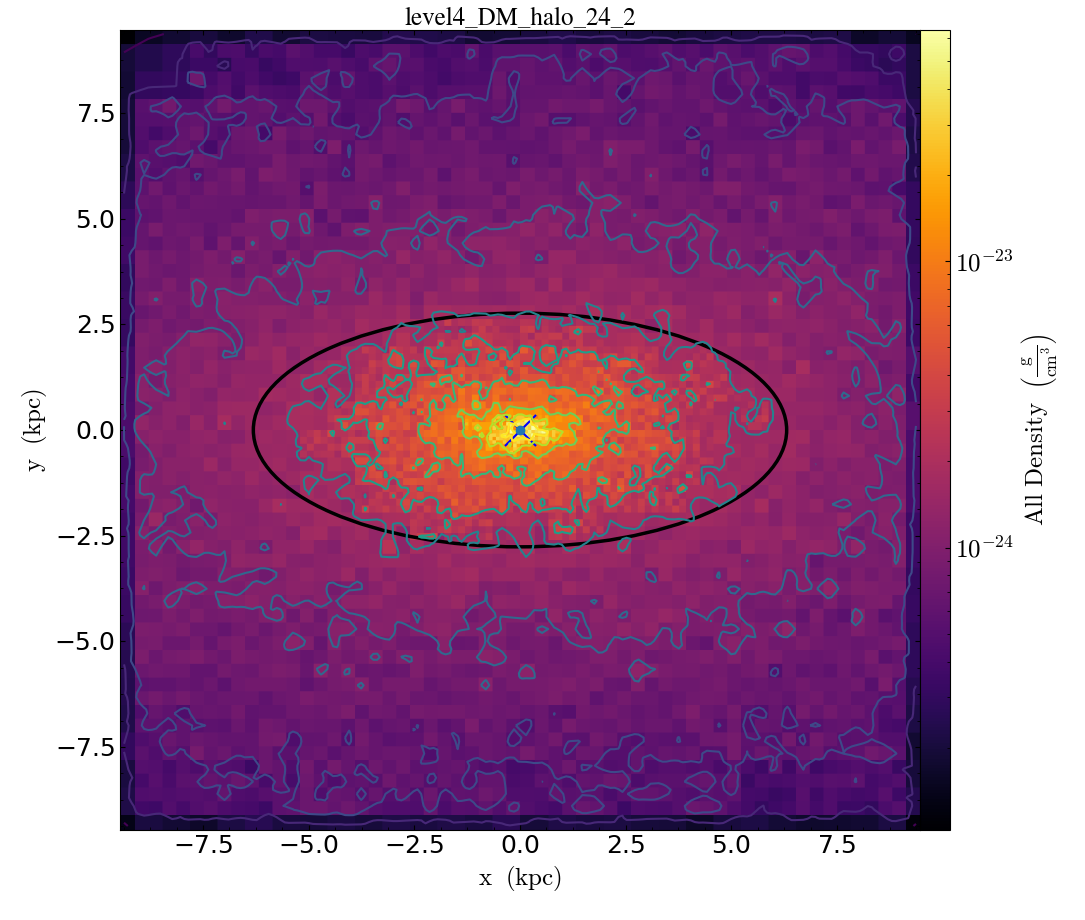
\includegraphics[width=0.5\textwidth]{level4_DM_halo_24_2.png}}  
  \hfill
  \subfloat[DMO simulation. Shape at large
    radius.]{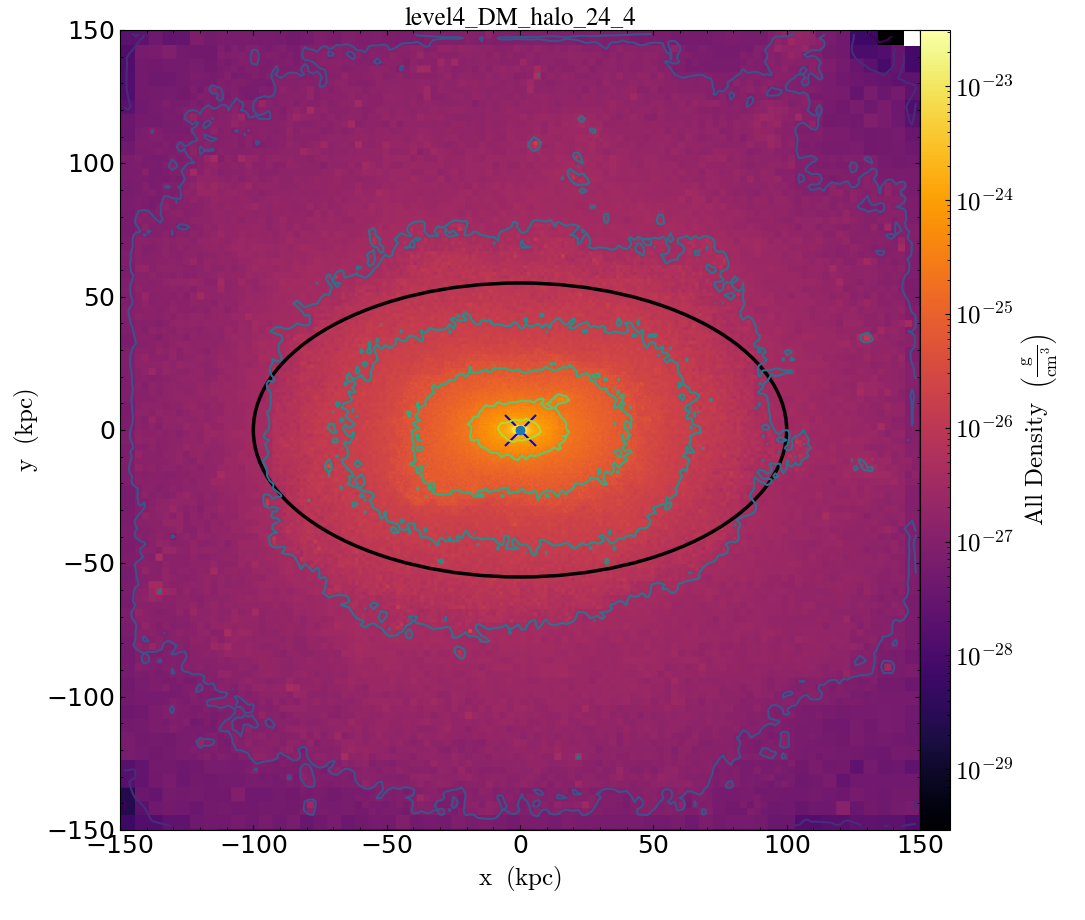
\includegraphics[width=0.5\textwidth]{level4_DM_halo_24_4.png}}  
  \hfill 

  \subfloat[MHD simulation. Shape at small
    radius.]{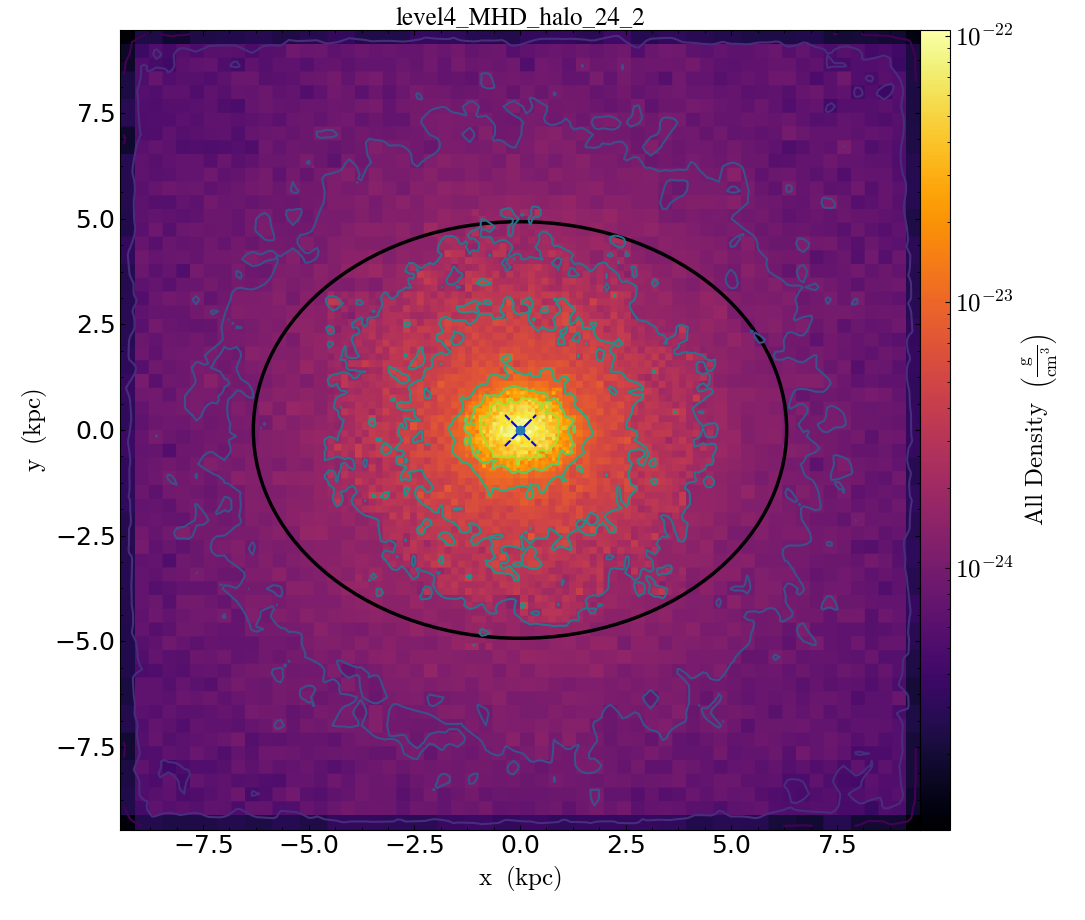
\includegraphics[width=0.5\textwidth]{level4_MHD_halo_24_2.png}}  
  \hfill
  \subfloat[MHD simulation. Shape at large
    radius.]{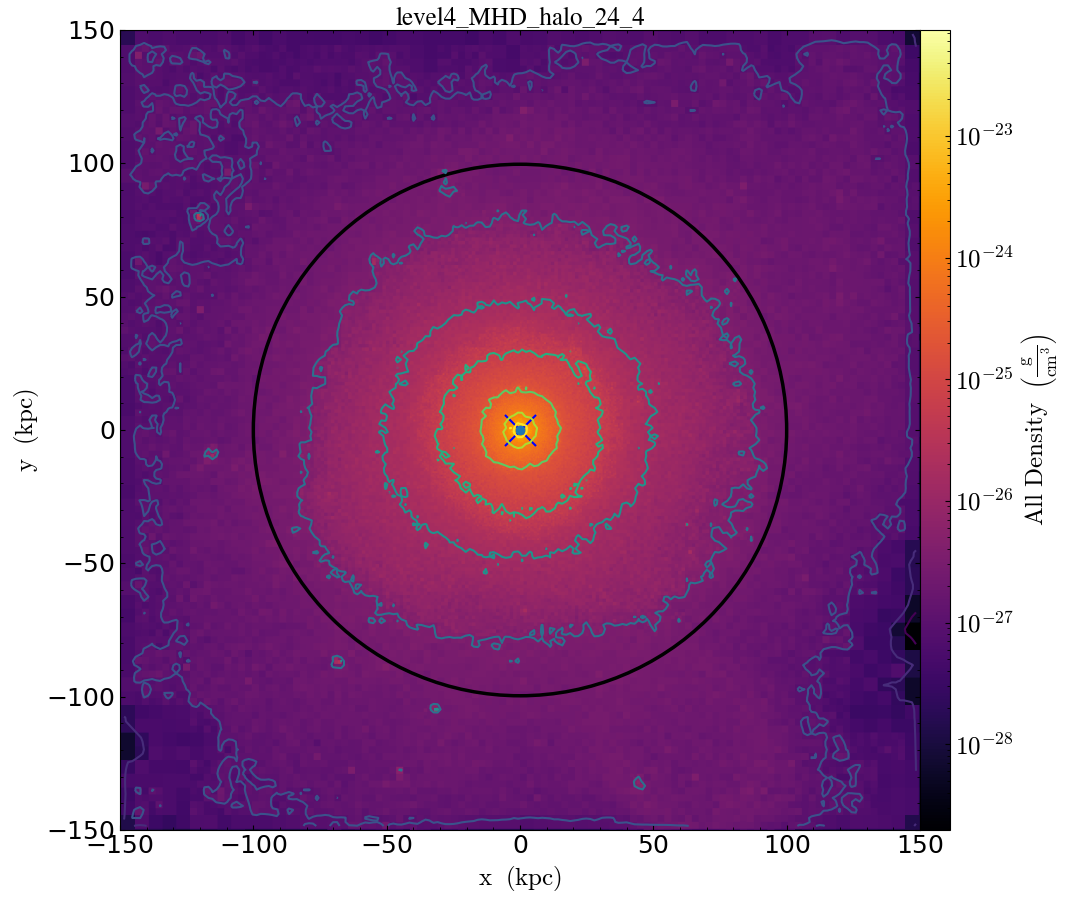
\includegraphics[width=0.5\textwidth]{level4_MHD_halo_24_4.png}}  
  \hfill 
  \caption{DM density in logarithmic scale within a slice of one tenth
    of the virial radius.
    The cut is perpendicular to the short axis of the inertia tensor ellipsoid.
    The black ellipses show the results of the fitting procedure
    described in Section \ref{sec:method}. 
    Upper/lower panels correspond to DMO/MHD simulations, respectively.
    Left/right panels show data at small/large radii, respectively.
    This plot showcases the most noticeable effect in all halos
    across the Auriga simulations: haloes are rounder at all radii
    after baryonic physics is included.}
\label{fig:slices}
\end{figure*}


 
\begin{figure*}
\begin{center}
\subfloat[DMO simulations.]{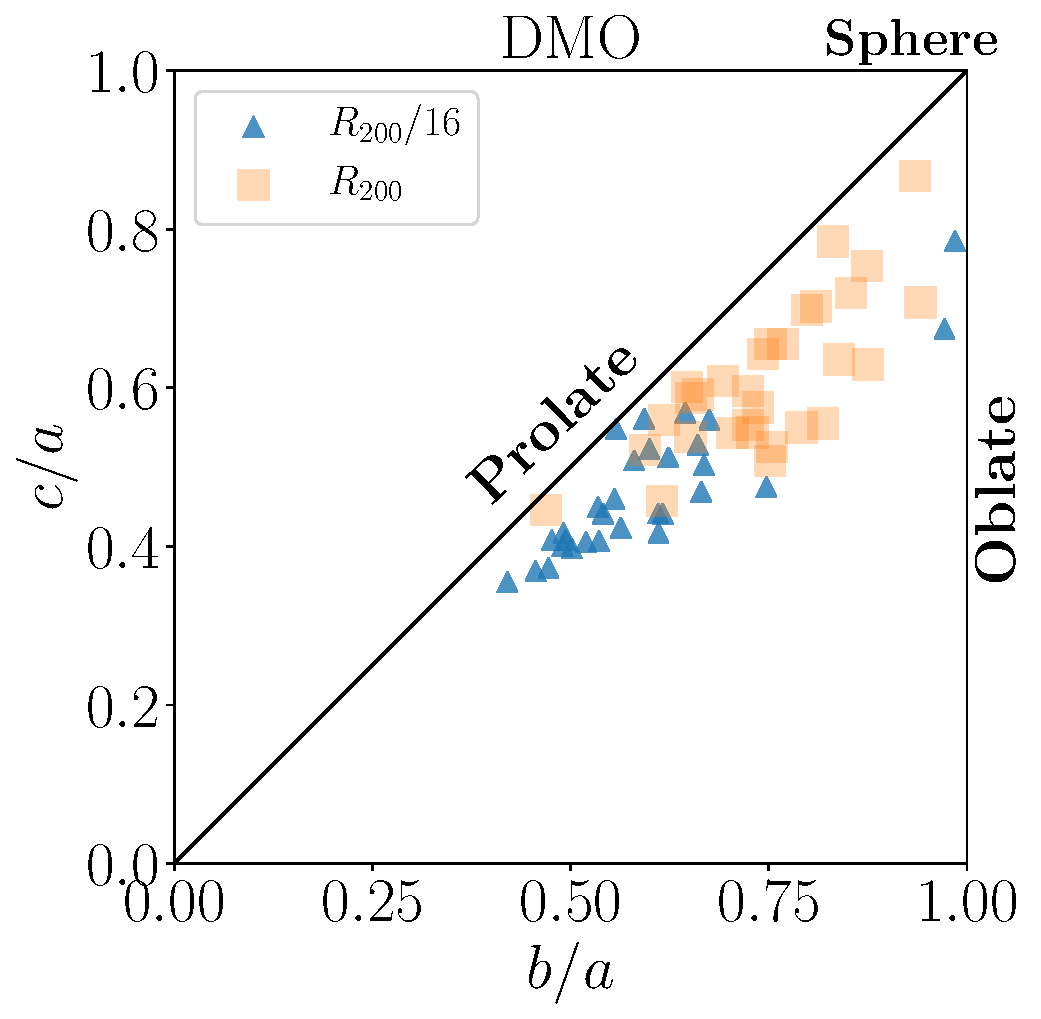
\includegraphics[width=0.8\columnwidth]{Lvl_4_Triax_Plane_DM.pdf}}
\subfloat[MHD simulations.]{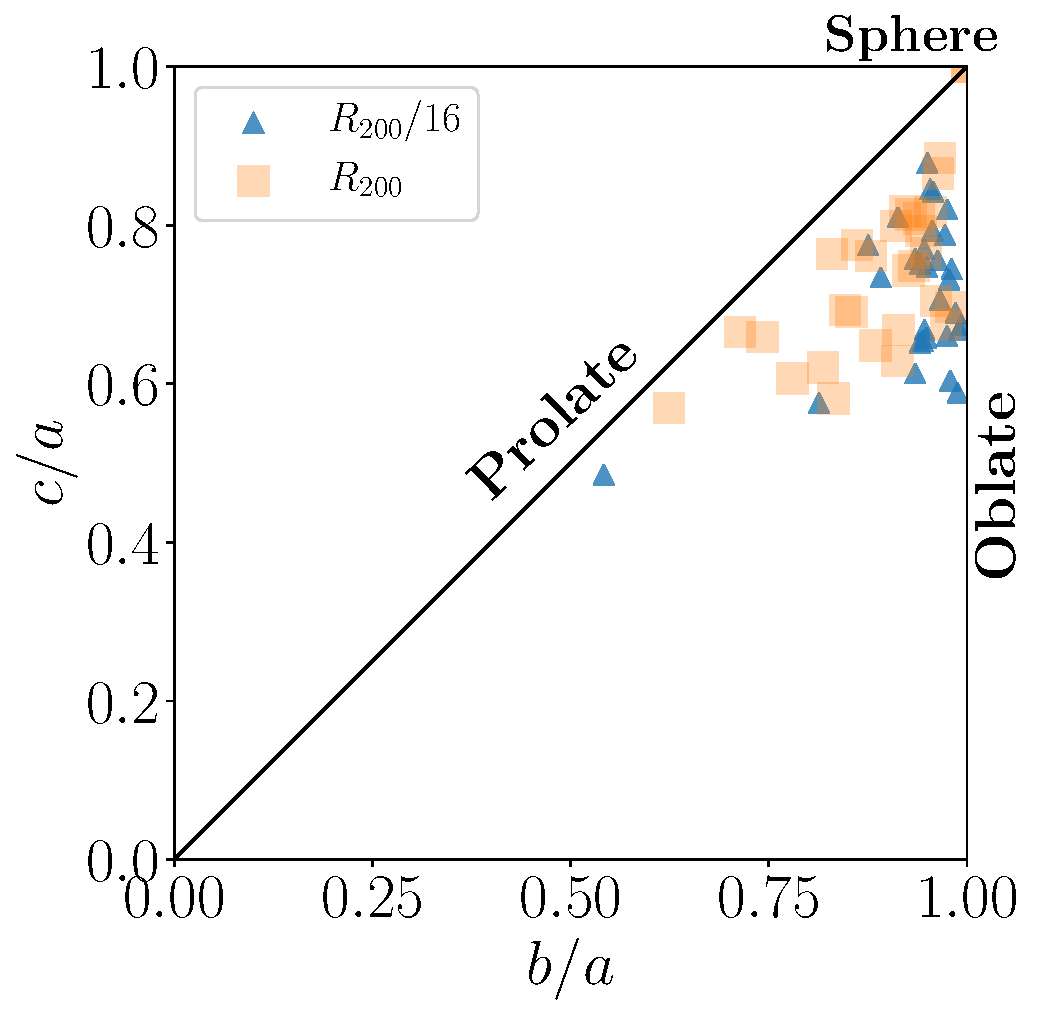
\includegraphics[width=0.8\columnwidth]{Lvl_4_Triax_Plane_MHD.pdf}}
\end{center}
\caption{Axial ratios for all simulated halos.
  Left/right panel corresponds to DMO/MHD simulations, respectively.
  Triangles (squares) represent the measurements at $R_{200}/16$
  ($R_{200}$) that correspond to physical distances of $14\pm 1$ kpc
  ($230\pm 15$ kpc).
  Here we visualize three main population trends.
  First, in DMO simulations halos are rounder in the outskirts
  than in the inner part.
  Second, halos in MHD are rounder than its DMO counterparts.
  Third, halos in MHD are rounder in the inner regions than in
  the outskirts (opposite to the DMO trend).}
  \label{fig:triaxiality_plane}
\end{figure*}


\begin{figure*}
\subfloat[DMO simulations.]{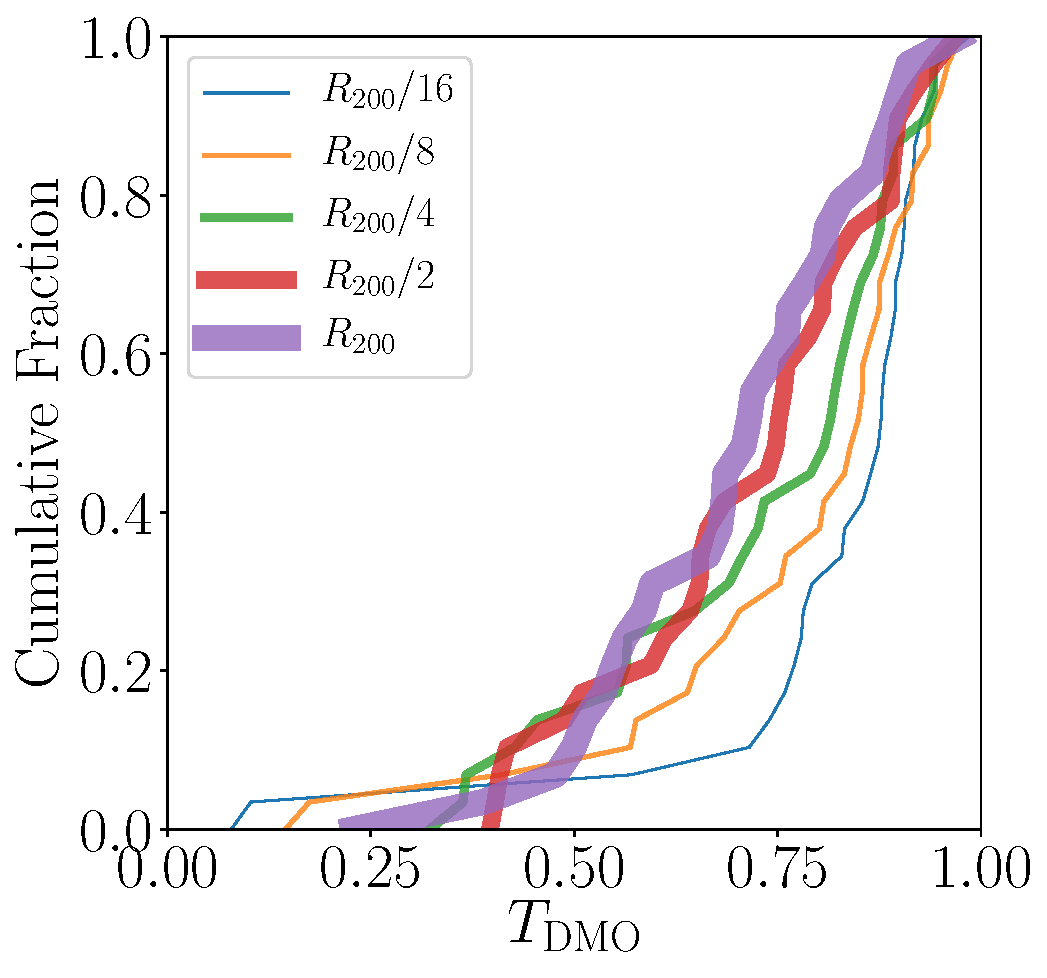
\includegraphics[width=0.8\columnwidth]{triaxialiy_distro_DM.pdf}}
\subfloat[MHD simulations.]{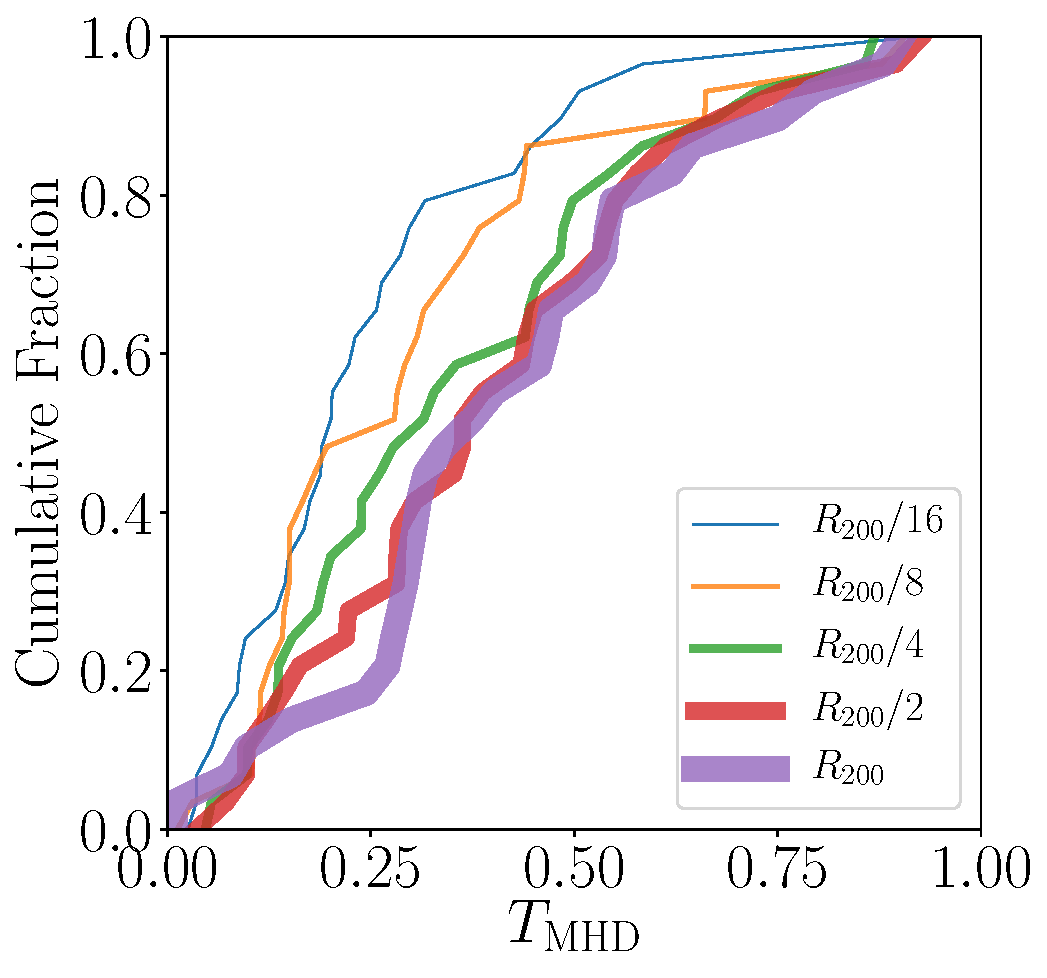
\includegraphics[width=0.8\columnwidth]{triaxialiy_distro_MHD.pdf}}
\caption{Triaxility cumulative distribution at five different radii.
  Right/left panel corresponds to DMO/MHD simulations, respectively. 
  In DMO simulations the median triaxiality at all radii is larger
  than $2/3$. Furthermore, the triaxility increases as one moves
  towards the inner part of the halo.
  In MHD simulations these trend reverses.
  The median triaxility at all radii is smaller than $1/3$ and the
  halo is less triaxial as on moves towards the stellar disc.}
\label{fig:triaxial_cumulative}
\end{figure*}


\begin{figure}
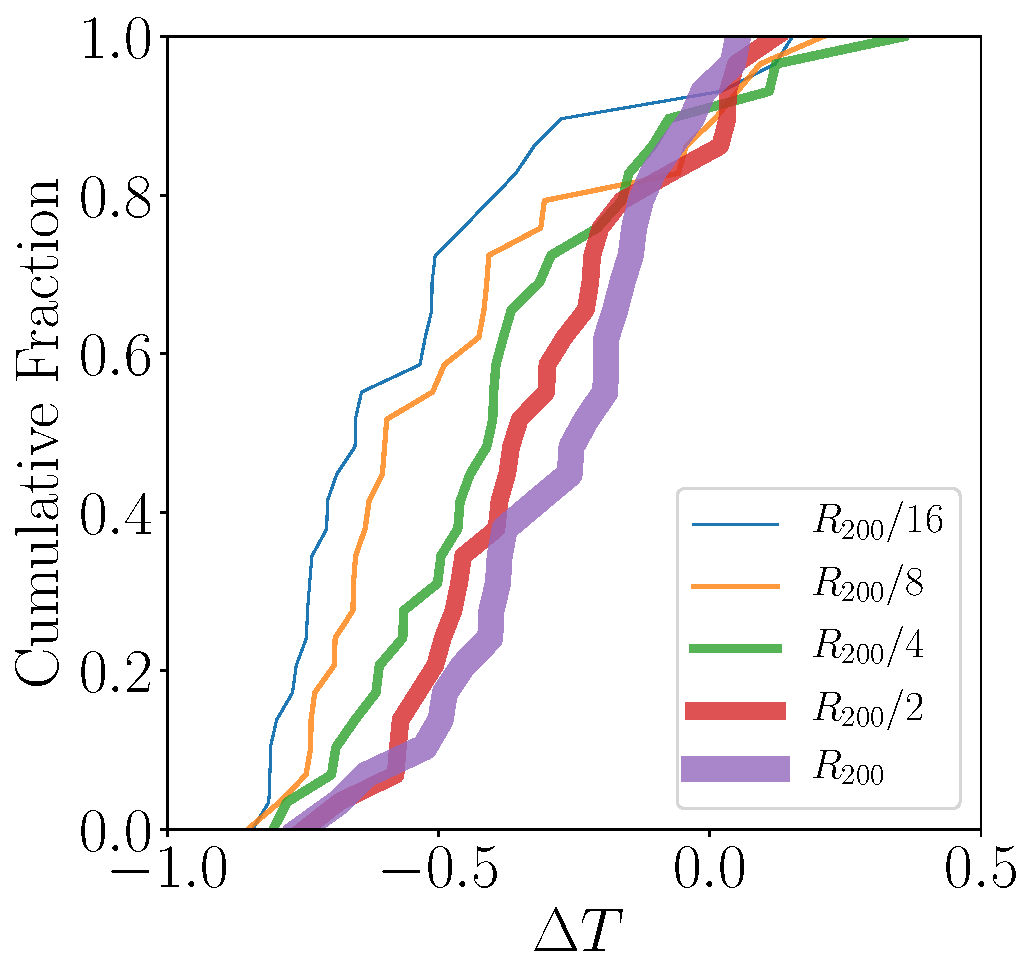
\includegraphics[width=0.9\columnwidth]{delta_triaxiality_distro.pdf}
\caption{
  Cumulative distribution for the changes in triaxility in simulations
  with different physics, $\Delta T=T_{\rm MHD}-T_{\rm DMO}$.
  At the virial radius all halos become less triaxial in the MHD
  simulations, the change is stronger towards the halo center.
  Only a small fraction of the halos ($\sim 1/15$) presents the
  opposite trend of becoming more triaxial towards the center.}
\label{fig:delta_triaxial_cumulative}
\end{figure}



\begin{figure*}
\begin{center}
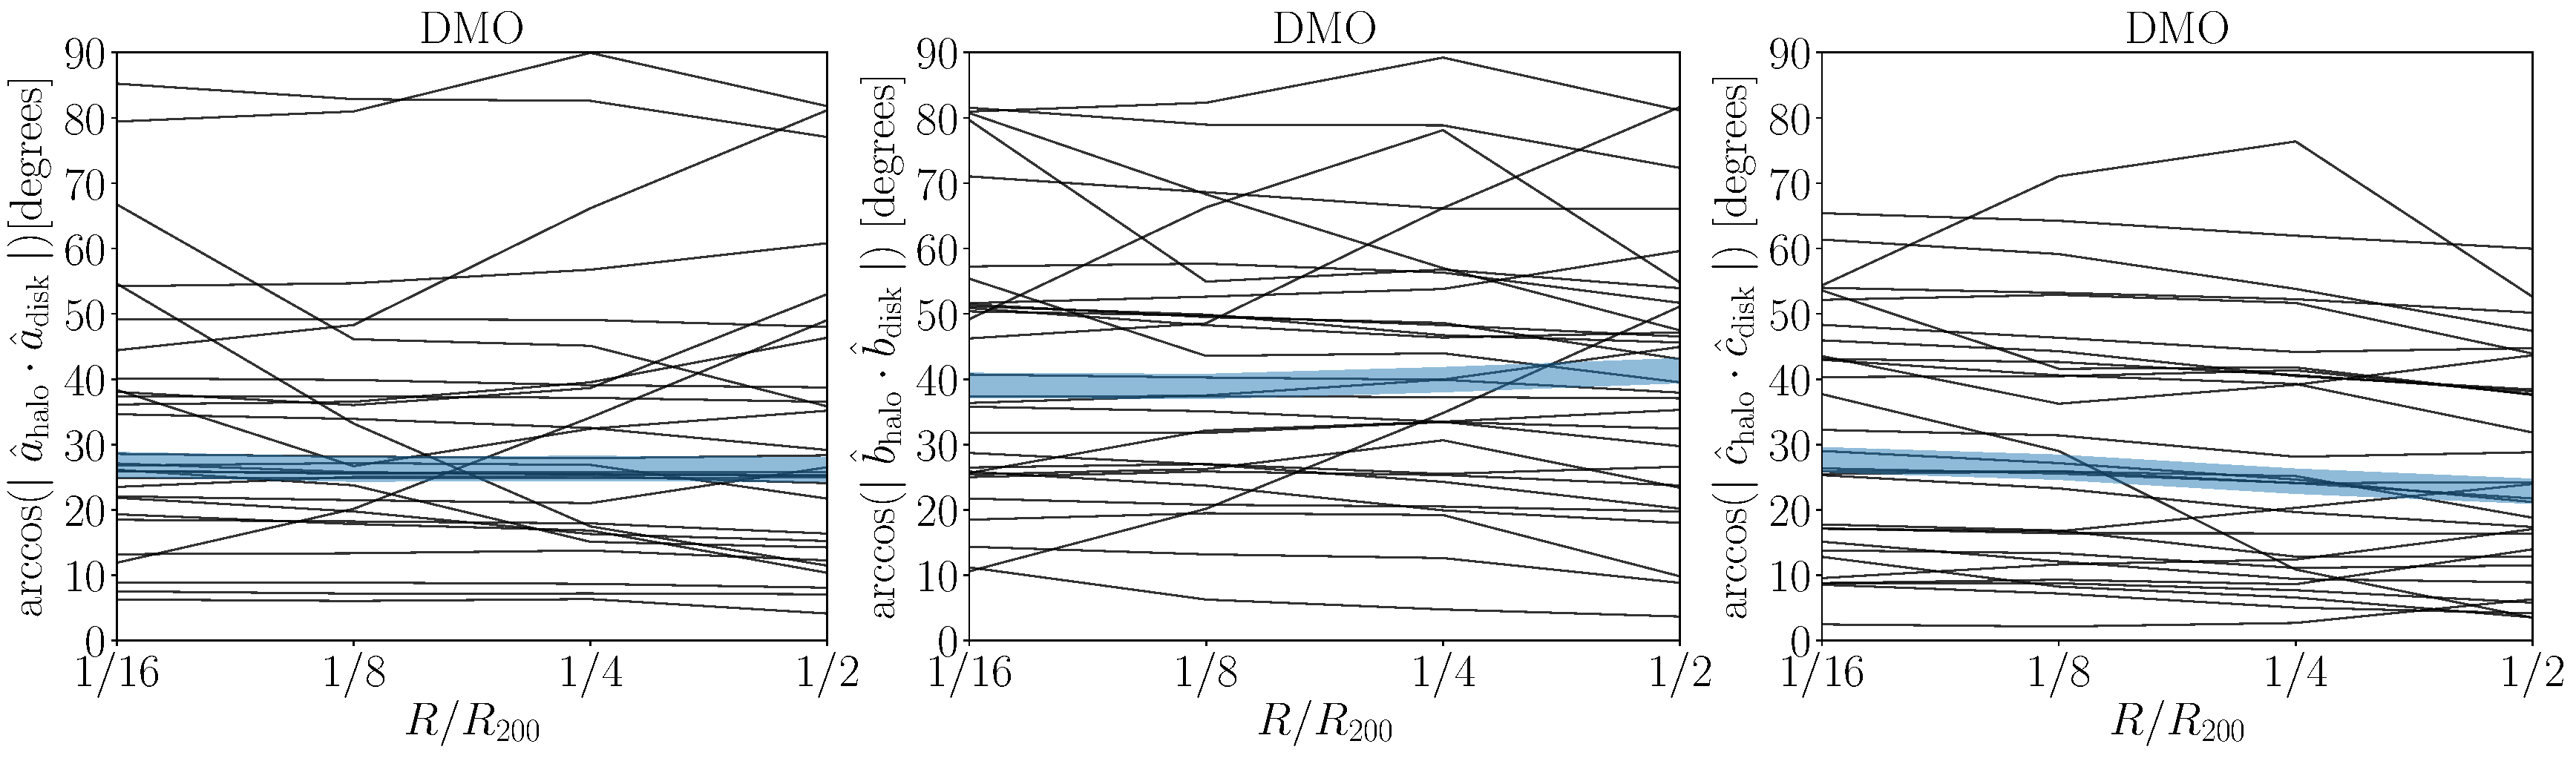
\includegraphics[width=1.0\textwidth]{angles_alignment_DM.pdf}
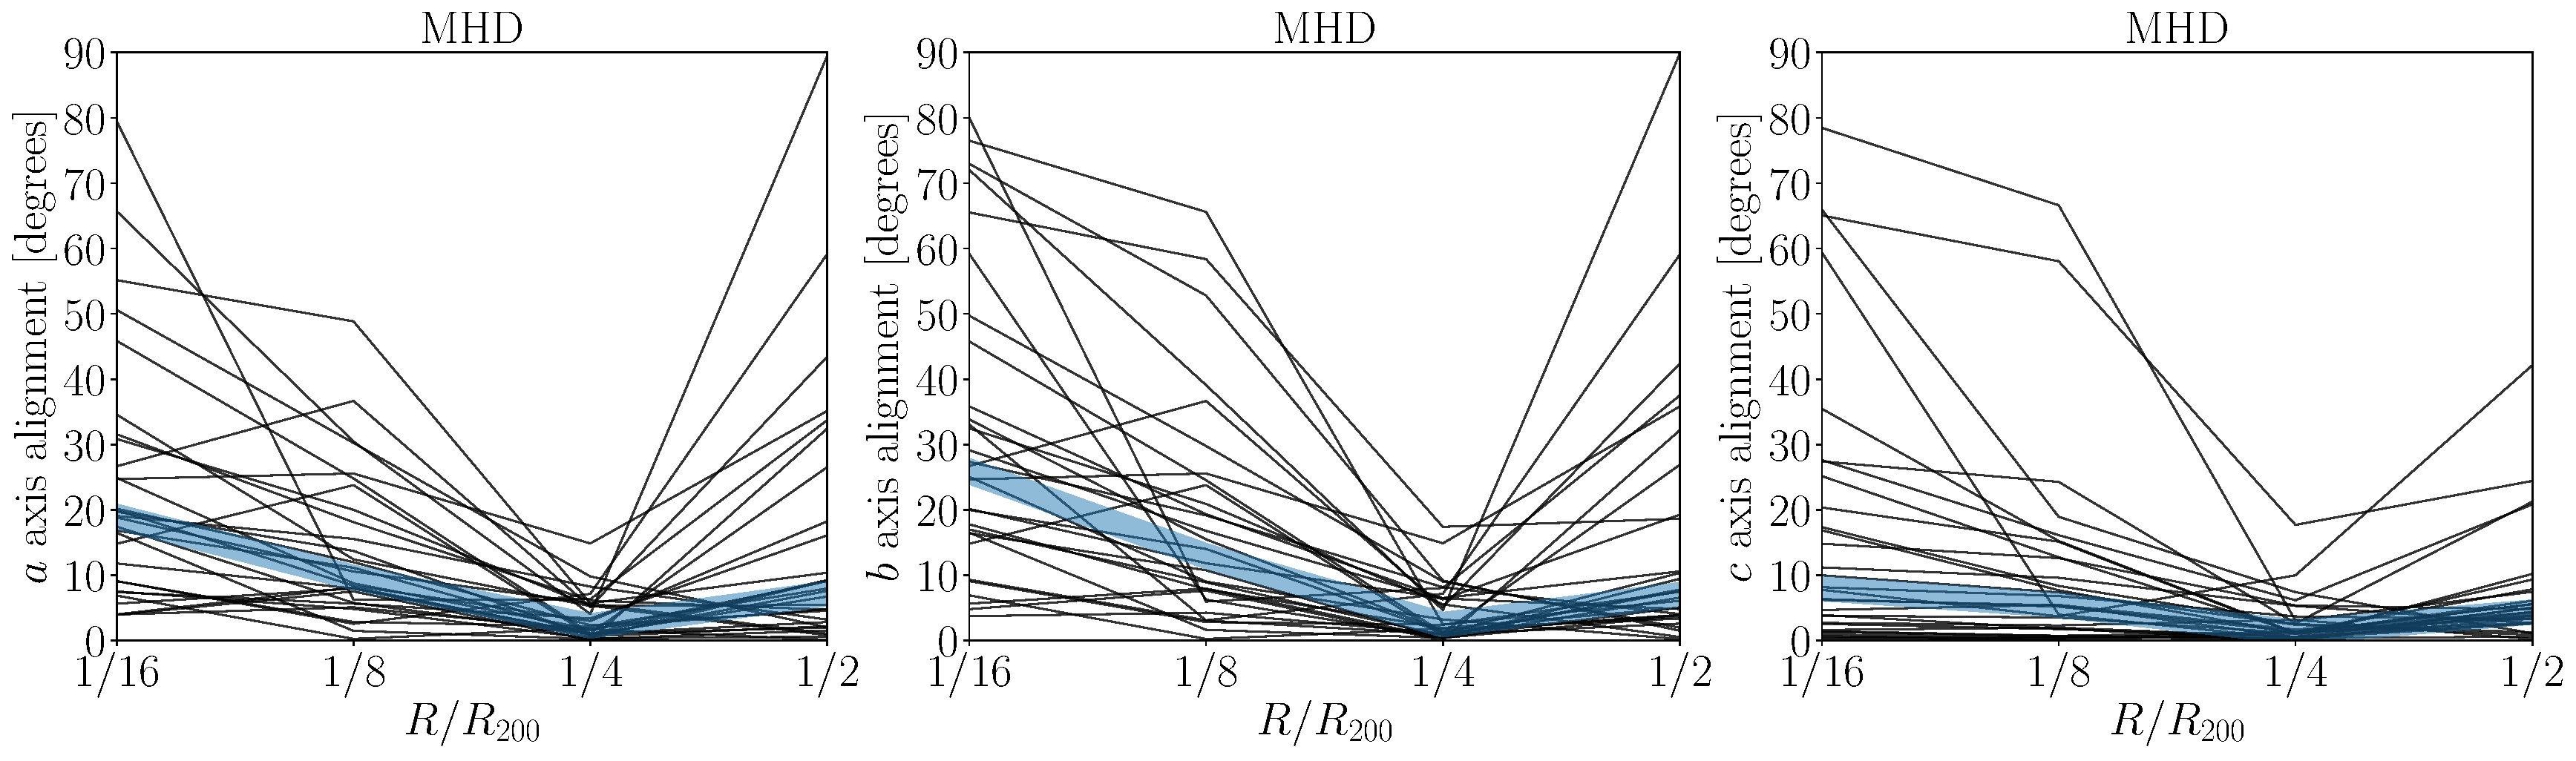
\includegraphics[width=1.0\textwidth]{angles_alignment_MHD.pdf}
\end{center}
\caption{Angles between the principal axis of the dark matter halo
  shape and the stellar disc shape as a function of the radius at
  which the halo shape directions are measured.
  Each panel compares the alignment of the corresponding
  major/middle/minor axis.
  Thin lines correspond to each one of the thirty halos in the sample
  while the thick line traces the median value at every radius.
  In the upper row the haloes come from the DMO simulation, 
  showing that the directions in the ellipsoids describing the shape
  are constant as a function of radius for the most part of the sample.
  In the lower row the haloes come from the MHD simulation providing a 
  self-consistent comparison with the stellar discs. 
  In this case the dark matter shells twists significantly in a
  noticeable fraction of the haloes.
  Interestingly, an almost perfect halo-disc alignment happens across
  the sample at an intermediate radius of $0.25R_{200}$ ($56\pm
  4$kpc). 
}
\label{fig:cumulative_alignment}
\end{figure*}


\begin{figure*}
\begin{center}
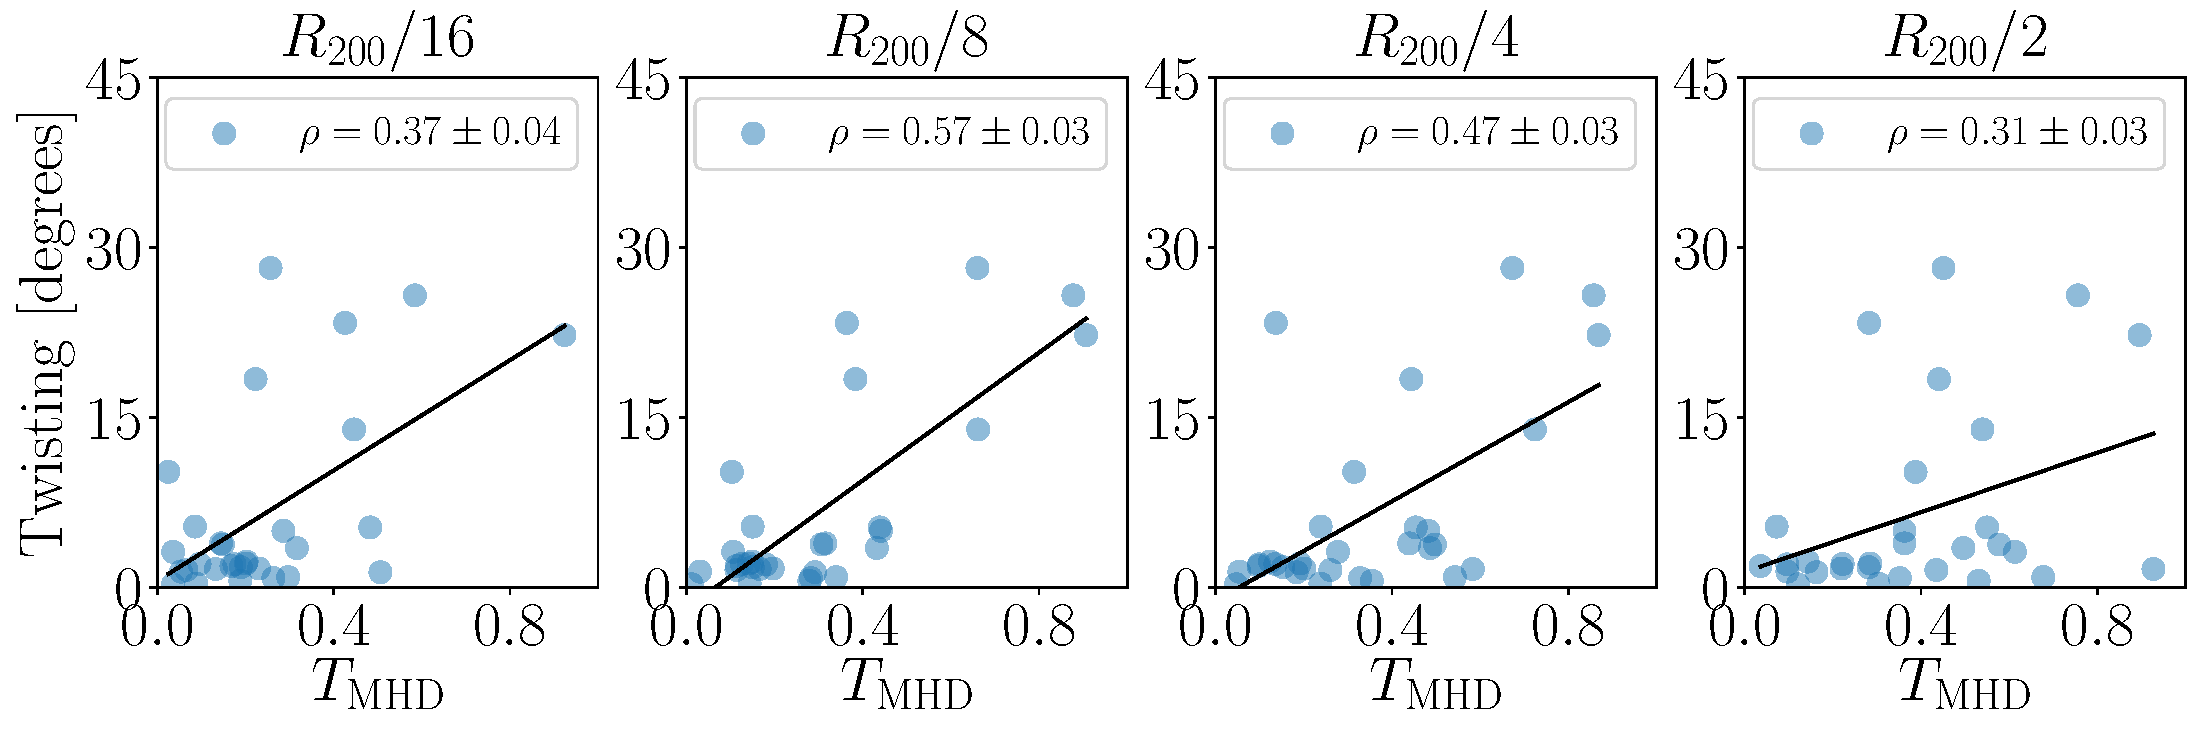
\includegraphics[width=1.0\textwidth]{correlations_twisting_triaxiality_MHD.pdf}
\end{center}
\caption{Twisting in the halo-disc alignment (measured as the standard deviation
  of the alignment angles between two minor shape axis)
  as a function of the halo triaxialiy at the radius indicated
  in each panel's title.
  The label with the $\rho$ value corresponds to the Spearman's rank
  correlation coefficient while the line shows the result of the
  minimum squares fit to the data.
  Twisting does not correlate with triaxility in the same way at every
  radii. The strongest correlation appears around $0.12R_{200}$ ($28\pm2$ kpc).} 
\label{fig:alignment_correlations}
\end{figure*}



\begin{figure*}
\begin{center}
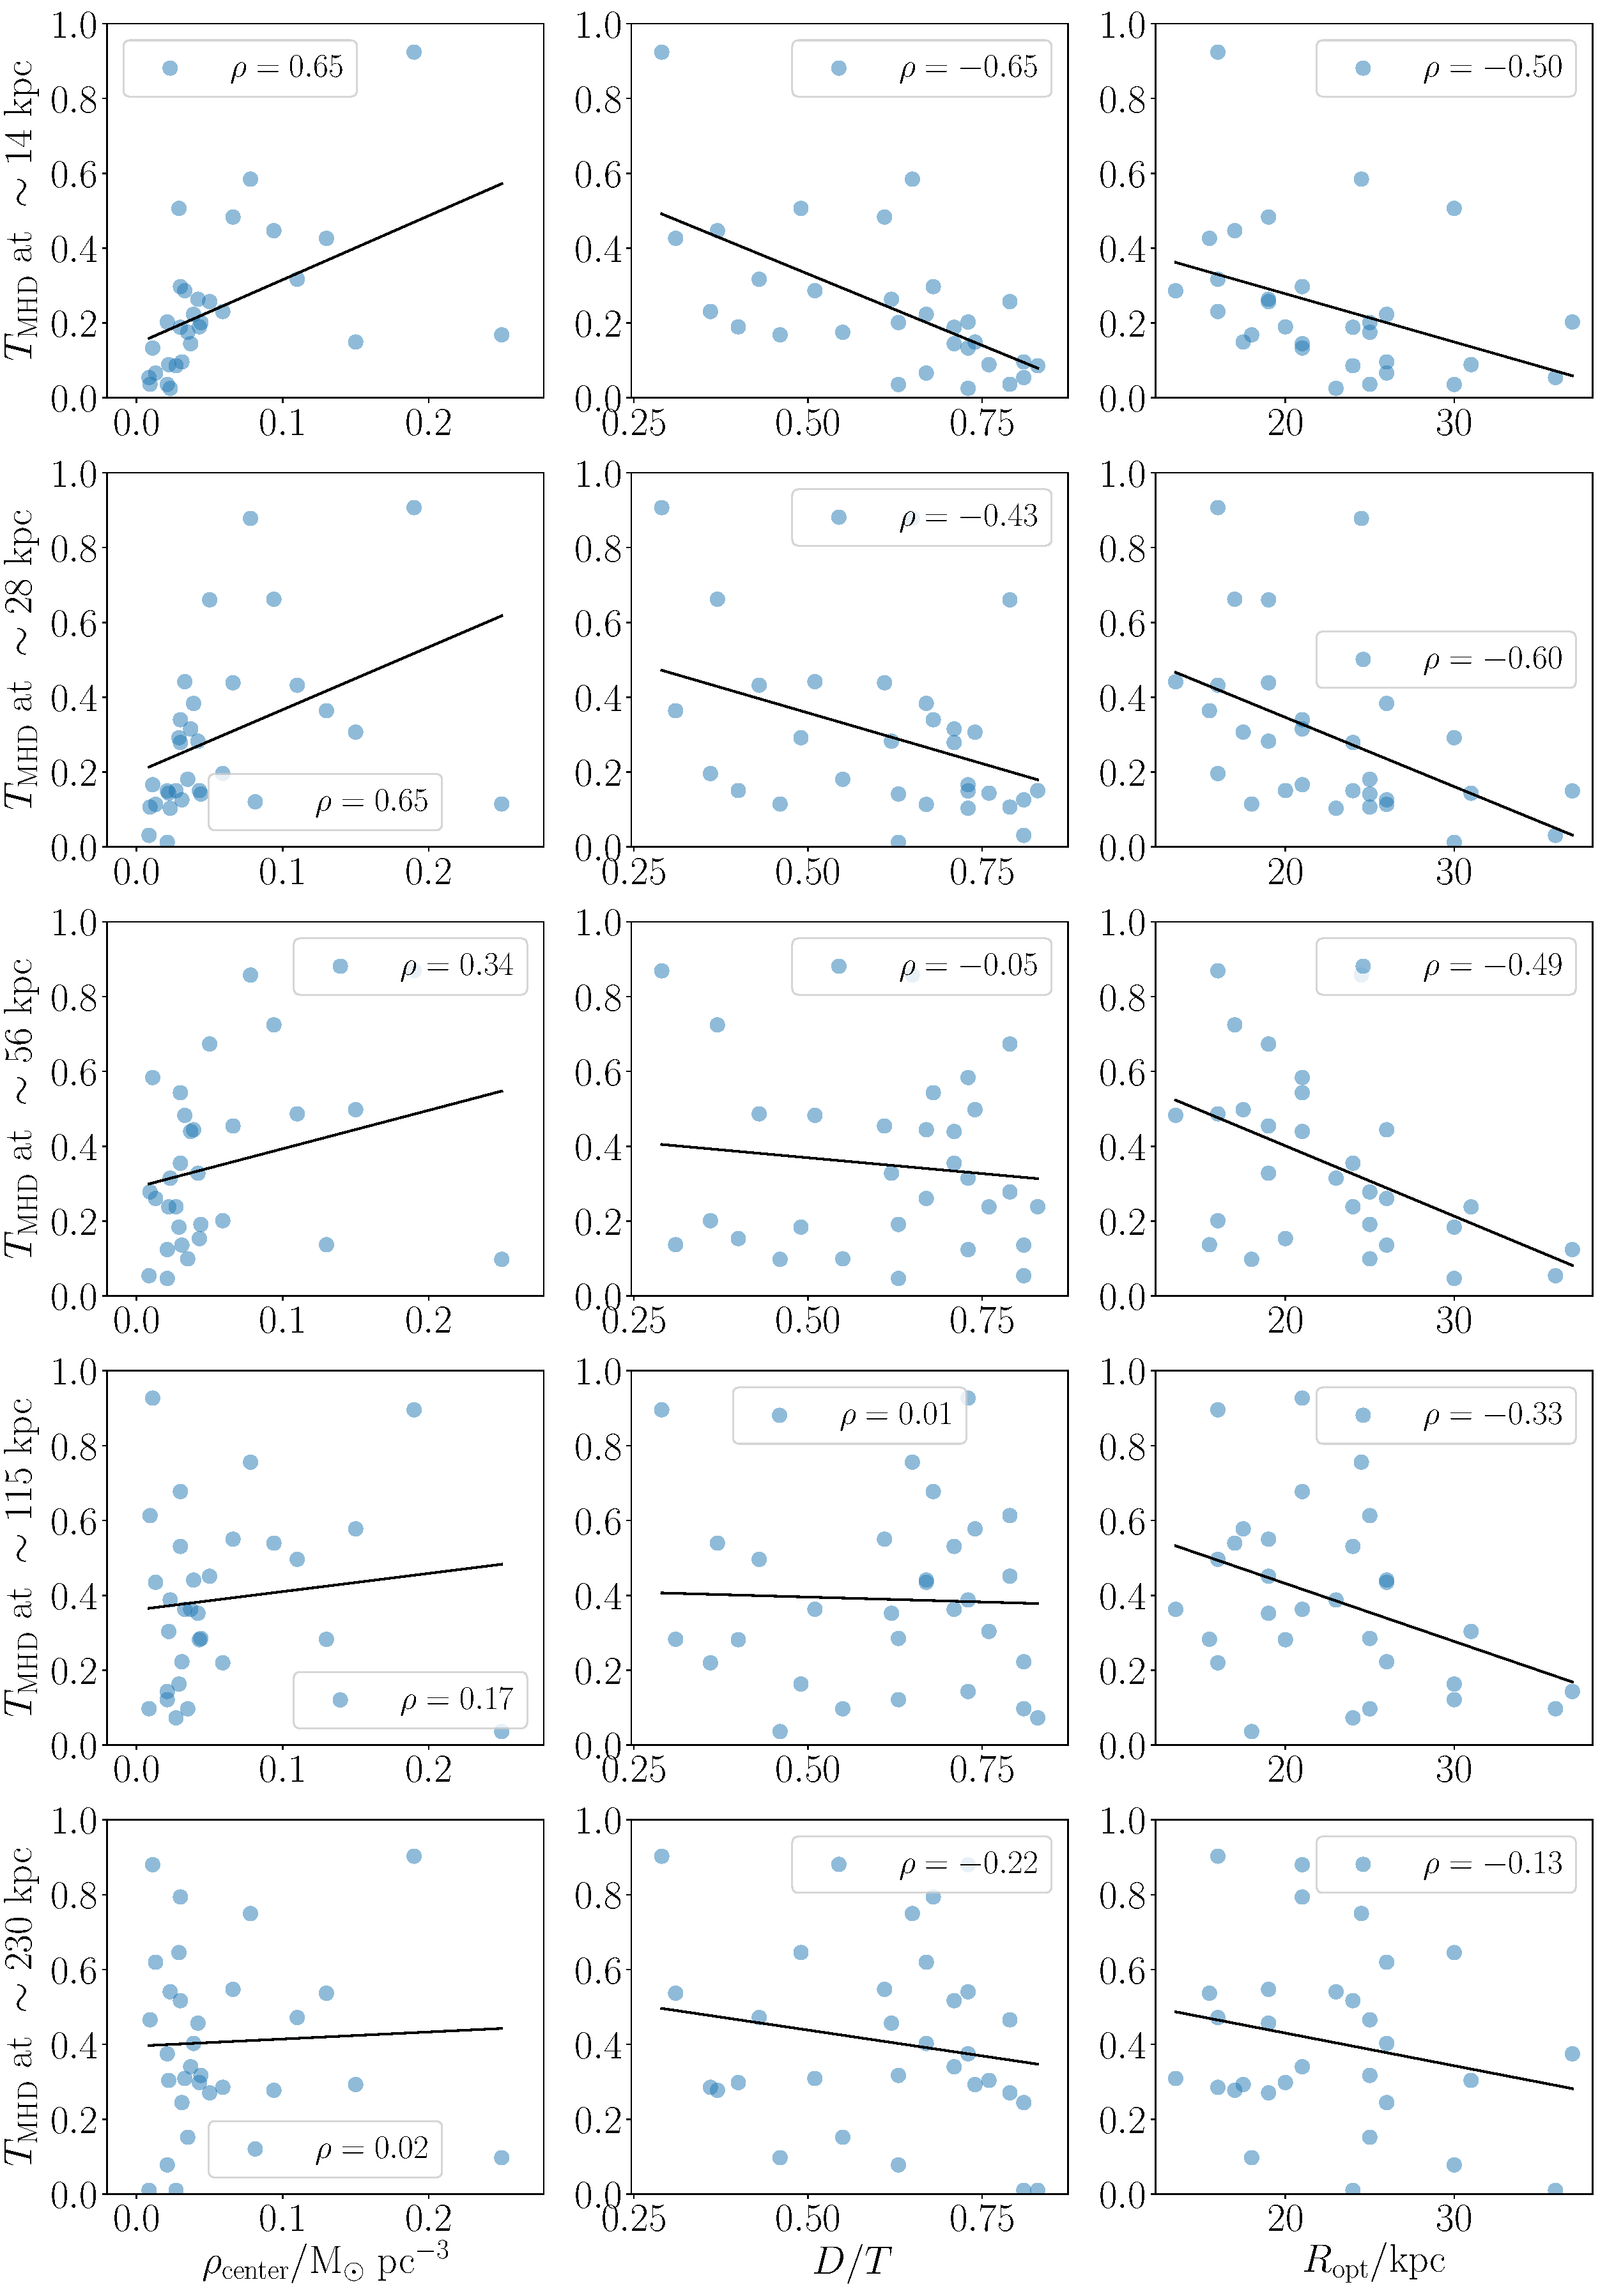
\includegraphics[width=0.8\textwidth]{correlation_T_MHD_disc.pdf}
\end{center}
\caption{Correlations between the halo triaxility at different radii
  and baryonic disc properties. 
  The label with the $\rho$ value corresponds to the Spearman's rank
  correlation coefficient.
  The line is the best minimum squares fit to a line.
  The x-axis in the first column is the gas density at the center of
  the galaxy with in a sphere of radius  $1$ kpc \citep{Pakmor17};
  the second column shows the disc to total mass ratio and the last
  column includes the disc optical radius defined to be the radius at which the
  $B$-band surface brightness drops below 25 mag arcsec$^{-2}$ \citep{auriga}.
  The largest correlations are found for the two smaller radii
  ($0.06R_{200}$ and $0.12R_{200}$).
  Extended and massive stellar discs with a low gas content at its
  core are correlated with low dark matter triaxilities.
  The correlation decreases as one approaches larger radii.}
\label{fig:disc_correlations}
\end{figure*}


\begin{figure*}
\begin{center}
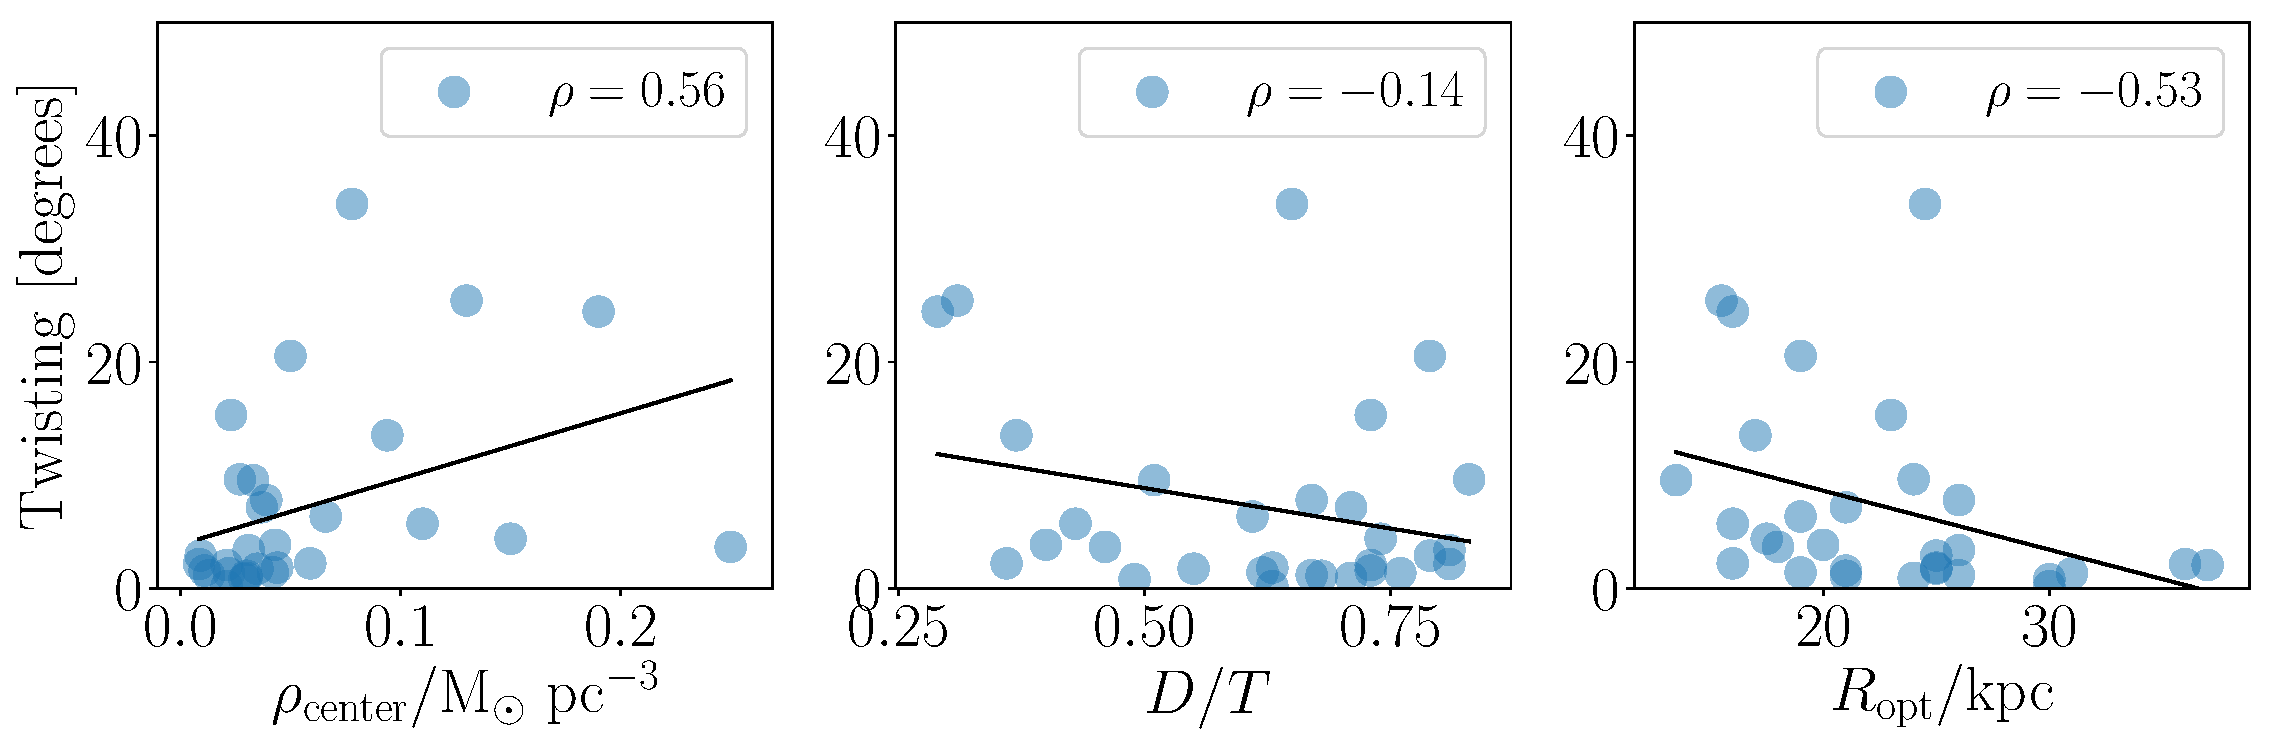
\includegraphics[width=0.9\textwidth]{correlations_angles_alignment_MHD.pdf}
\end{center}
\caption{Twisting in the halo-disc alingment as a function of the same
  baryonic disc properties in Figure \ref{fig:disc_correlations}.
  The label with the $\rho$ value corresponds to the Spearman's rank
  correlation coefficient.
  The line is the best minimum squares fit to a line.
  In this case the disc to total mass ratio does not correlate stronly
  with the alignment twisting.
  The gas density at the center and the disc optical radius still show
  a strong correlation.}
\label{fig:alignment_correlations}
\end{figure*}




\section{Halo Shape Measurement}
\label{sec:method}

The DM halo shape is an estimate of either the isopotential or
isodensity surfaces.   
Observational inference models usually estimate the 
isopotential contours which are probed by tracers (gas, stars), while
simulations work with the isodensity contours which can be directly
calculated from particle positions.  
Furthermore, the density contours in thin shells are very sensitive to
the presence of small satelites.  
For this reason we measure the shape by taking
volume-enclosed particles, rather than shell-enclosed.  
This method yields results in good agreement to the isodensity
contours for radii $\leq 140$ kpc as explored by
\citep{VeraCiro11}.  


In particular, we measure the shape using the reduced inertia tensor
\citep{Allgood06},  

\begin{equation}
I_{ij} = \sum_k \frac{x_k^{(i)}x_k^{(j)}}{d^2_k},
\label{eq:inertia}
\end{equation}

where the particle positions are measured from the minimum of the
gravitational potential in each halo and each is weighted by the k-th
particle distance $d_k^2=x_k^2+y_k^2+z_k^2$.

The diagonalization of this tensor yields the eigenvectors and
eigenvalues that represent an ellipsoidal dark matter halo.
The axis lenghts of this ellipsoid $a\geq b \geq c$ are the square
root of the ${\bf I}$ eigenvalues and the direction of the principal
axis are the corresponding eigenvectors 

We start the calculations taking into account particles within a
sphere of radius $R_{\rm initial}$ and then recharacterize the
triaxial parameters 
by taking into account particles within an ellipsoid of semi-axes
$r,r/q,r/s$ and re-scaled distance $d^2=x^2+(y/q)^2+(z/s)^2$, where $q
= b/a$ and $s=c/a$ are the previously calculated axial ratios. 
We repeat this process until the average deviation of semi-axes is
less than $10^{-6}$.  
After convergence we define a unique radius $R$ as the geometrical
mean of the axial lenghts $R=(abc)^{1/3}$.
We use this radial coordinate $R$ to parameterize the spatial changes
in halo shape we report in the following sections.
This is the same method used to estimate the halo shape in the DM-only
Aquarius simulations \citep{VeraCiro11}. 

Following the convergence criterion by \cite{VeraCiro11} in DM only simulations
we restrict the measurement of the ellipsoidal parameters to radii
between $2$kpc and $R_{200}$ where  $R_{200}$ corresponds to the radius
computed enclosing a sphere with 200 times the critical density of the
Universe. 
This scale is similar to the gravitational smoothing lenght for
stellar particles. 
For this reason, in order to make the DM halo shape results comparable
against stellar disc shape measurements, we report our DM halo shape
results above $10$ kpc.
For the shape of the stellar disk we include all stellar particles
within a radius of $0.01R_{200}$, that is $\approx 23$kpc. 

In our results we express the radius as a fraction of $R_{200}$ in
order to have a self-consistent dimensionless radius scale across all
halos. 
Given the small variance across halos, each dimensionless radius is associated with
a physical value with a mean value and a standard deviation.
For instance, over the 30 halos in the sample, the dimensionless
radius $R_{200}$ corresponds to a physical distance of $230\pm 16$
kpc.  


\section{Results}
\label{sec:results}

\subsection{Triaxiality}

In the DMO sample we find that halos are rounder with increasing
radius.
The upper panels in Figure \ref{fig:slices} illustrate this effect.
The contours show a projected DM slice while the ellipsoid corresponds
to the full 3D shape determination. 
There we see a highly ellipsoidal halo shape at radii $\sim 3$kpc
that becomes less triaxial at $\sim 50$ kpc.

We summarize this trend in Figure \ref{fig:triaxiality_plane} by
plotting the results of all the 30 halos in the DMO sample.
The left panel shows every halo in the $c/a$-$b/a$ plane at
two different radii $R_{200}/8 (\sim 20$kpc$)$ and $R_{200}$. 
The outer part of the halo is systematically rounder than its inner
region. 
Nevertheless the halo shape can still be considerated to be prolate at
all radii. 

A different picture presents itself in the MHD sample.
There all halos become rounder at all radii than its DMO
version.
The lower panel in Figure \ref{fig:slices} can be directly compared to
its MHD counterpart; there we observe how at large radii the halo
becomes oblate and almost spherical. 
The right panel in Figure \ref{fig:triaxiality_plane} shows the
results for the 30 halos in the MHD sample.

In Figure \ref{fig:triaxial_cumulative} we summarize the results at
different radii using the cumulative distributions for the 
triaxility parameter $T$ defined as 

\begin{equation}
T=\frac{a^2-b^2}{a^2-c^2}.
\label{eq:triaxiality}
\end{equation}

The left panel of Figure \ref{fig:triaxial_cumulative} shows that in
the DMO sample the triaxility has a median larger than $2/3$ (a
typical value that marks the transition from triaxiality to
prolateness) at all radii. 
Furthermore this median value increases as we move towards the inner part of the
halo.
The right panel shows how the correlations in the MHD simulations go
in the opposite direction with respect to DMO result.s
There the median triaxility is alwas smaller than $1/3$ (a typical
values that marks the transition from triaxility to prolateness) and this
median value decreases as we move towards the inner part of the halo.

We now quantify this change in triaxility at the level of individual halos.
We compute $\Delta T\equiv T_{\rm MHD}-T_{\rm DMO}$ to quantify the
change between the triaxility in the MHD and the DMO simulation.
Figure \label{fig:delta_triaxial_cumulative} shows the cumulative
distribution at the same radii as in
Figure \label{fig:delta_triaxial_cumulative}.  
From this Figure we observe that at $R_{200}$ all the halos have
reduced its triaxility include baryonic physics.
At smaller radii this general trend continues, although there is a
small fraction ($\approx 1/15$) of halos that slightly increased their
triaxility with MHD physics. 
However, this small fraction correspond to halos that already were
outliers in the DMO sample and had triaxilities around $1/3$,
considerably lower than its parent sample.


\subsection{Halo-disc alignments}

A common assumption in dynamical models of the MW DM halo is that
its minor axis is perfectly aligned with the stellar disc minor axis.
Although it is a reasonable assumption to guarantee the stability of
the galactic disc in simplified models of isolated galaxies, this
might not perfectly hold in an explicit cosmological context. 
To examine the degree of validity of this assumption we study in this
subsection the alignment between the eigenvectors of the inertia tensor of
stellar particles within $0.1R_{200}$ ($\sim 23\pm 2$ kpc) and the
eigenvectors of the dark matter halo shape.

In Figure \ref{fig:cumulative_alignment} we summarize our main results
regarding these alignments with the halo shape measured at five
different radii.
The upper row shows the alignment of the halos in the DMO simulations
with the stellar disc in the MHD simulations.
The main objective of this measurement is to calibrate the radial
evolution of the DM halo shape. 
We find that the DM shape remains constant with radius.

The upper row in Figure \ref{fig:cumulative_alignment} shows 
the alignments between the major/intermediate/minor axis of the
disk and the halo as a function of the dimensionless radius at which
the halo shape was measured.
The upper row shows the angle between the DMO halo and the stellar
disk in the MHD simulation.
This comparison help us to measure how the shape directions in the
dark matter shells change with radius.
For the bulk of the sample the lines are horizontal.
Only two halos in the sample show a significant change in alignment in
on the three shape axis.

The lower row in Figure \ref{fig:cumulative_alignment} shows th
results for the MHD simulations.
The most striking feature of this plot is that around the radius of
$0.25R_{200}$ there is an almost perfect halo-disc alignment measured
in three shape axis.
Above and below this radius the degree of alignment changes.
We find the strongest missalignments at a radius of $0.06R_{200}$ when
the median and the standard deviation of the alignment angles between
the minor/median/major axis are $18\pm18$, $25\pm22$ and $7\pm21$
degrees, respectively;  at $0.25R_{200}$ these values drop to $2\pm3$,
$2\pm4$ and $1\pm 3$ degrees, respectively

This changing alignment as a function of radius can be seen as a
twisting in the shape ellipsoids. 
As we are dealing with oblate halos $b/a\approx 1$ and the
directions corresponding to the medium and major axis could be subject
to noise.
For this reason, in order to better quantify the twisting for each
halo we take the standard deviation of the angle between the two minor
axis, which should be less succeptible to noise.
With this measurement, twisting becomes a global property of the halo,
as the standard deviation is measured over the different radii at
which we have quantified the alignment.

Figure \ref{fig:alignment_correlations} shows the correlation between
twisting at the four different radii at which we have measured the
alignments. 
The median, mean vand standard deviation of the triaxiliy are $3$, $7$ and $8$
degrees, respectively.
The correlation between twisting and triaxility also changes with
radius as measured by the Spearman's rank correlation coefficient.
The largest correlation shows with the halo triaxility measured at
$0.12R_{200}$. 
The most important consequence of this changing degree in correlation
is that twisting cannot only be explained by large triaxiality values
and a possibly noisy determination of the shape axis.

\subsection{Correlation with baryonic disc properties}


The presence of baryons produce rounder dark matter halos than its DMO
counterpart.
To better understand this relationship we quantify the correlation
between halo shape with baryonic disc properties.  
Looking into the measurements already reported by \cite{auriga} and
\cite{Pakmor17} we find three baryonic quantities that have the
strongest correlation with DM halo triaxiality: the central gas
density in a sphere of radius $1$kpc, the disc to total mass ratio and
the optical radius. 

Figure \ref{fig:disc_correlations} shows the correlations of
these quantities with the triaxility at five diferent radii.
We use the Spearmen's rank correlation coefficient to quantify the
correlation strength.
We find that the strongest correlations are found with the halo shape
measured at radii smaller than $0.12R_{200}$.
The  trend is such that halos with large triaxiality correlate with
high gas density and stellar discs with low mass and small size. 
In turn, massive and large stellar discs within with low density of
gas in its core correlate with low halo triaxiliaty. 

The halo shape also twists in the presence of baryons, as opposed to
the situation in DMO simulations where the shape is coherent as a
function of radius.
In Figure \ref{fig:alignment_correlations} we show the correlation
between twisting and the same baryonic properties that showd a high
degree of correlation with the triaxility.
In this case the disc to total ratio does not have a significant
degree of correlation.
Instead, the disc optical radius and the gas density at the core are
the most correlated. 
The correlation is such that extended stellar discs with a very low
gas density at its core show the most coherent halo shapes.  

\section{Discussion}
\label{sec:discussion}


The first effect that we put in evidence in this paper is the effect
of baryons in producing rounder DM halos.
This effect has been already widely reported in the literature.
It has been found that the strength of the change depends on the
numerical resolution, the gas cooling implementation and the
models describing star formation and stellar feedback
\citep{Kazantzidis04,Bailin05,Debattista08, Bryan13, Butsky16, Chua19, Artale19}.  
The key concept unifying these results is that the baryon distribution
influences and correlates with the dark matter halo shape. 
Indeed, as we presented in the previous section on the correlations
with disc properties, we find that the broad tendency is that extended
massive stellar discs correlate with spherical dark matter
distributions.  

In contrast, there are fewer studies reporting on the halo-disc
alignment as a function of radius.
\cite{JingSuto02} reported a shell alignment twisting in their dark
matter only simulations as measured in the direction changes of large
and medium shape axis. 
They only had three high resolution MW-like halos (with
$\sim 10^{6}$ inside the virial radius) and could not make a
statistical statement about the impact of this effect.
However, they see the twisting as an artifact resulting from high values of the
$b/a$ ratios that make the determination of the medium axis noisy.
For that reason we measured the twisting using the minor axis
alignments, however they do not report these alignments.


\cite{Bailin05} used seven hydrodinamical simulations studied the disc
halo alignmnent as a function of radius.
For radii smaller than $0.1R_{200}$ they find a strong alignment
between the two minor axis of the halo and the disc. 
For larger radii the angle between the components changes showing a
weak correlation between the two components. 
\cite{Debattista13} performed a study on the disc-halo aligment
performing controled experiments on three different halos to study
changes the evolutionary change that drive the minor axis in the disc
and the halo to be aligned, their study by construction focuses only
on radii around $0.1R_{200}$.
Nevertheless, similarly to \cite{Bailin05}, they also report a strong
alignment in the region where the disc dominated. 
In conclusion, the twisting in the dark matter halo shapes seems to be
a feature already reported in the literature with smaller samples than
the one we use here. 
The strongest point of depart is that in our case the alignments do
not grow stronger as one approached the disc.
It is very likely that the detailed radial dependence of the twisting
depends on the hydrodynamics and feedback implementations. 

We now use the results reported by \cite{LM10} and \cite{Bovy16}
to place our results in an observational context.
\cite{LM10} used observations of the Sagittarius tidal stream to
constrain the shape of the gravitational potential.
Their point of depart is that previous studies that assumed an
axisymetric galactic potential were not able to fit all the available
dynamic constraints for the Sagittarius stream, therefore making
necessary the use of a rigid triaxial potential with coaxial potential
ellipsoids for the dark matter component.  
Their results constrain the triaxility of this potential
component. 
They also translate ther results into a triaxiality of the density
contours (that could be compared against our results)
 to be $(c/a)=0.44$ and $(b/a)=0.97$ at a radius of $\sim 40$kpc. 
They do not report any uncertainties for these two values. 
Looking at their plots for the quality of fit criterion as a function
of dark halo axial scales (their Figure 5), we choose a conservative $10\%$
relative uncertainty.
One surprising element in their results is that  the major axis of the
halo shape is perpendicular to the stellar disc plane.  

The results by \cite{Bovy16} have the same general approach but use
instead the GD-1 \citep{2006ApJ...641L..37G} and Pal 5 \citep{2009AJ....137.3378O}
streams to constraint the shape of the dark matter component of the
galacic halo potential.
They use general models with many degrees of freedom for the galactic
potential in order to measure to what extent these two streams are sensitive
to the triaxiality of the dark matter halo component.
The DM component is written directly as a triaxial density profile
with coaxial ellipsoids and the corresponding potential is found by
numerical integration.
They find that the width of the Pal 5 stream constraints $b/a\approx
1$ and therefore fix it to be $b/a=1$ exactly.
Using that value they report their most stringent constrain of
$c/a=0.93\pm0.16$ at a radius of $\approx 19$kpc from the galactic
center. 

Figure \ref{fig:observations} shows an explicit comparison in
the $c/a$-$b/a$ plane of our results in MHD simulations against the
results by \cite{LM10} and \cite{Bovy16}.
We find six MHD halos with $b/a<0.93$ and $c/a>0.77$ that could be
considered consistent with their shape constraints  by \cite{Bovy16}, while
only one outlier DMO halo is consistent with those constraints.
In contrast, none of the simulated halos (MHD nor DMO) is consistent
with the results \cite{LM10}. 
The change of triaxility with radius in our simulations cannot account
for these two extremely different shape constraints at different
radii. 


The results by \label{LM10} could then place the dark matter halo of our Milky
Way as an extreme outlier in the $\Lambda$CDM model. 
This extreme prolateness also correlates with the extreme triaxiality
of the 11 classical satellites of the MW ($c/a\approx 0.2$, and
$b/a\approx0.9$) measured at larger radii, with an spatial
distribution  also oriented perpendicular to the MW plane, another
highly unusual feature in the $\Lambda$CDM \citep{2018MNRAS.478.5533F}. 


\begin{figure*}
\begin{center}
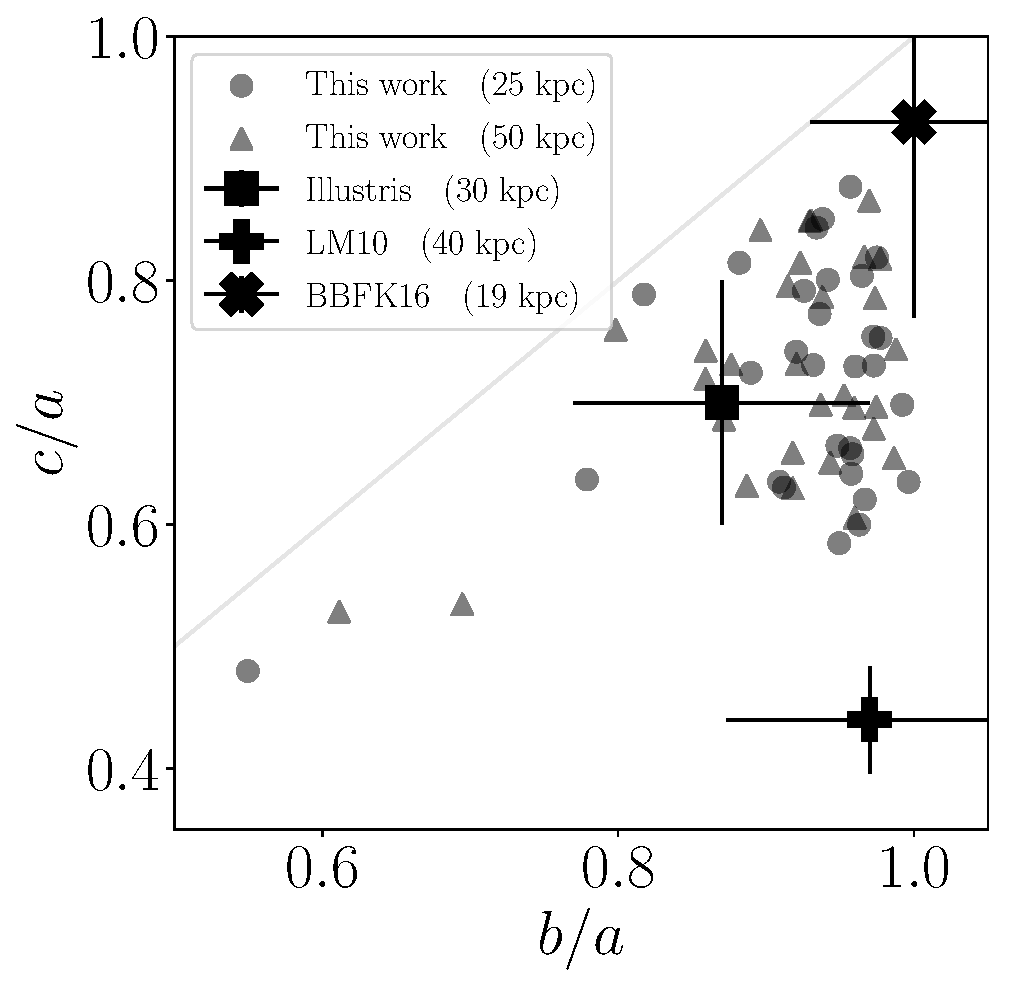
\includegraphics[width=0.7\textwidth]{triaxiality_observations.pdf}
\end{center}
\caption{Comparison of our results against 
observational constraints for the 
dark matter halo shape in the Milky Way by \citet{LM10} (LM10) and
\citet{Bovy16} (BBFK16).   
We find that  1/5 of the halos in the MHD  sample are consistent with
the constraints by \citet{Bovy16}.
In contrast, none of the halos in the MHD and DMO seems to be
consistent with the results by \citet{LM10}.}
\label{fig:observations}
\end{figure*}

\section{Conclusions}
\label{sec:conclusions}

In this paper we measured the shape of 30 isolated Milky Way sized
dark matter haloes simulated in the Auriga project using the zoom-in
technique. 
The halos were with two different setups:
dark matter only (DMO) simulation and full magnetohydrodynamics (MHD)
including star formation and feedback.
We used the shape measurement algorithm by \cite{Allgood06} on the
dark matter halos of these simulations to quantify the halo shape as a
function of radius and the degree of aligment between the stellar disc
and the halo. 

We find that MHD halos are rounder than DMO halos at every radius.
MHD halos tend towards more oblate, sometimes almost spherical, shapes
($T<1/3$), while DMO halos tend towards more prolate shapes ($T>2/3$).  
The rounding effect is more noticeable as one moves closer to galactic
disc and strongly  correlates with baryonic properties of the disc
More precisely, the triaxility is smaller for extended and massive
stellar discs with low gas densities at its core.

We also measured the shape alignment of the halo with the stellar
disc at different radii.
At a radius of $0.25R_{200}$ the alignment is almost perfect and
degrades at smaller and larger distances.
In some halos the alignment betwen the stellar disc and dark matter
halo changes noticeably with radius. 
This alignment evolution implies a radial twisting between the ellipsoids
describing the halo shape. 
We quantify this twist with the standard deviation of the angle
between the two minor axis at radii below $\leq 0.5R_{200}$ and find
that the twisting strongly correlates with the disc size and the core
gas mass density, there is only a weak correlation with the disc to
total mass ratio.

We compared our results against two observational constraints for the
dark matter halo shape of the Milky Way. 
The constraints are at two different radii and come from different
observatinal tracers. 
We find that $20\%$ halos in the MHD simulations are consistent with
the constraints by \cite{Bovy16} at $\approx 19$kpc that correspond to
an almost spherical halo, while none of the halos, either in MHD or
DMO, has some overlap with the shape constraints by \cite{LM10} at
$\approx 40$kpc that is closer to oblate.  


Using dark matter only simulations \cite{VeraCiro11} suggested that
the current dark matter halo shape strongly correlates with the time
evolution of the halo as traced by the shape measured at the virial radius. 
This effect might no longer hold once baryons are included. 
The opposed trend of triaxiality in MHD simulation as a function of
radius to the DMO simulations together with the twisting effect in some of 
the halos seems to suggest that that historical buildup memory is not
stored in the halo at $z=0$.


A more complete understading of the influence of baryons on the
different properties we have measured will require at least two more elements.
First, an study on how the halo and the disc co-evolved as a
function of time. Second, a calibrating the effect of the cosmic web
(both dark matter and gaseous) on any evoluionary trend
\citep{2014MNRAS.443.1090F,2017MNRAS.469..594B,2019MNRAS.487.1607G} 
We finalize by suggesting that the twisting density shells we find in
some of the halos is feature that deserves to be explored in the
process of constraining shape parameters from tidal stream data.  The
inclusion of a parameterization describing this degree of twisting
might relax the conflict between the observational constraints and the
numerical results.  


\section*{Acknowledgements}
This project has received funding from the European Union's Horizon
2020 Research and Innovation Programme under the Marie
Sk\l{}odowska-Curie grant agreement No 734374. 

 \bibliographystyle{mnras}
 \bibliography{references}

\end{document}


